\documentclass{beamer}



\usepackage[ngerman]{babel}
\usepackage{default}
\usepackage[utf8]{inputenc}
\usetheme{Berlin}
\usecolortheme{beaver}
\uselanguage{ngerman}

\title{Korrespondenzproblem}
%\subtitle{Subtitle}
\author{Soeren Berken-Mersmann}
\institute
{
  DHBW Karlsruhe
}
\date{17. April 2015}
\subject{Theoretische Informatik}

\begin{document}
\frame{\titlepage}

\frame{
	\frametitle{Gliederung}
	
	\begin{enumerate}
		\item Postsches Korrespondenzproblem
		\item Simulation einer Turingmaschine
		\item Beweis der Nichtberechenbarkeit
		\item Beweise weiterer Probleme
	\end{enumerate}
}

\frame{
	\frametitle{Postsches Korrespondenzproblem}
	
	% Analogie von Dominosteinen verwenden, Bilder inkludieren.
	
	% Beispiele, einfach lösbare, und unlösbare
	% % Zuerst hier anschaulich darstellen was das Korrespondenzproblem ist
	% % Anschließend die allgemeine Beschreibung des Problems vorstellen
}

\frame{
	\frametitle{Postsches Korrespondenzproblem (formell)}
	
	\begin{block}{Definition des PKP}
	Gegeben sei eine endliche Menge an Wortpaaren $K = ((x_1, y_1), ..., (x_k, y_k))$, über dem Alphabet $\Sigma$ mit $x_i, y_i \in \Sigma$. Gibt es eine Folge von Indizes $i_1, i_2, ..., i_n \in {1, 2, ..., k}, n \geq 1$, so dass $x_{i_1},x_{i_2}, ... x_{i_n} = y_{i_1}, y_{i_2}, ..., y_{i_n}$.
	\end{block}
	
}

\frame{
	\frametitle{Simulation einer Turingmaschine}
	
	% Anwendungszweck? Simulation einer Turingmaschine
	
	Um die zu Beweisen, dass das PKP nicht berechenbar ist, werden wir eine Turingmaschine simulieren.\newline
	
	Dafür müssen wir zuerst den Rechenweg einer Turingmaschine formalisieren. \newline
} \frame {
	\begin{block}{Zustand einer Turingmaschine}
	\begin{center}
		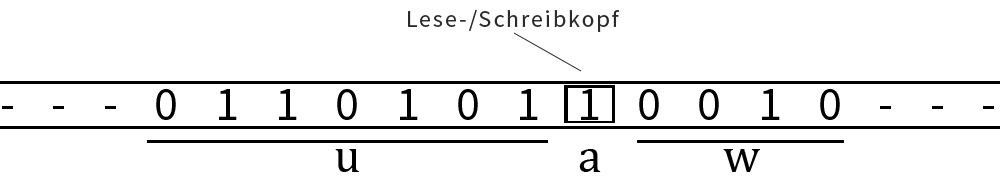
\includegraphics[width=0.85\linewidth]{./abbildungen/turing-snapshot}
	\end{center}

	\begin{itemize}
		\item Linkskontext: $u$
		\item Interner Zustand: $q$
		\item Gelesenes Symbol: $a$
		\item Rechtskontext: $w$
	\end{itemize}
	Somit lässt sich der Zustand $Q_t$ einer Turingmaschine zum Zeitpunkt $t$ durch die Folge $u_tq_ta_tw_t$ darstellen.
	\end{block}
} \frame {		
	\begin{block}{Rechenweg}
	Den Rechenweg einer Turingmaschine können wir als die Folge von Zuständen $Q_0, ..., Q_n$ vom Startzeitpunkt $t = 0$ bis zum Endzeitpunkt $t = n$ bei dem die Turingmaschine einen der Endzustände erreicht hat.
	% Formulierung überarbeiten 
	\end{block}
} \frame {	
	\begin{block}{Beispiel}
	Formalisierte Darstellung: $0110101,q_01,0010\sharp01101011,q_10,0010$ \newline
	Der Lesekopf liest eine $1$ und befindet sich in Zustand $q_0$, die Regel die Anwendung gefunden hat ist $q_01 \rightarrow q_10R$.
	\end{block}	
	\pause[2]
	\begin{block}{Simulation der Regel $q_10 \rightarrow q_11$}
%	$0110101q_010010\sharp01101011q_100010\sharp\pause[2]0\pause[3]1\pause[4]1\pause[5]0\pause[6]1\pause[7]0\pause[8]1\pause[9]11q_1\pause[10]0\pause[11]010\pause[12]\sharp$\newline
%	$\pause[1]0110101q_010010\sharp\pause[2]0\pause[3]1\pause[4]1\pause[5]0\pause[6]1\pause[7]0\pause[8]1\pause[9]1q_10\pause[10]0\pause[11]010\pause[12]\sharp$
	$0110101q_010010\sharp01101011q_100010\sharp\pause[3]0\pause[4]1\pause[5]1\pause[6]0\pause[7]1\pause[8]0\pause[9]1\pause[10]11q_1\pause[11]0\pause[12]010\pause[13]\sharp$\newline
	$\pause[2]0110101q_010010\sharp\pause[3]0\pause[4]1\pause[5]1\pause[6]0\pause[7]1\pause[8]0\pause[9]1\pause[10]1q_10\pause[11]0\pause[12]010\pause[13]\sharp$
	\end{block}
	
} \frame {
	% An dieser Stelle dann die genauen Regeln vorstellen (s. Wegener)
	% Die wichtigen im Detail (Kopier-Regeln, Zustandsübergangsregeln)
	% Und die "unwichtigen" nennen
	
}

\frame{
	\frametitle{Beweis der Nichtberechenbarkeit}
	
	% % Halteproblem
	% % Reduktion
}

\frame{
	\frametitle{Beweise weiterer Probleme}
	Seien $G_1$ und $G_2$ zwei kontextfreie Grammatiken, und $L_1 = L(G_1)$ und $L_2 = L(G_2)$ zwei daraus konstruierte kontextfreie Sprachen.
	
	\begin{block}{Eindeutigkeit}
	Ist $G_1$ eindeutig?
	\end{block}
	
	\begin{block}{Gleichheit}
	Ist $L_1 = L_2$?
	\end{block}
}

\frame{
	\frametitle{Eindeutigkeit}
	
	% % Beweis entsprechend führen
}

\frame{
	\frametitle{Gleichheitstest}
	
	% % Beweis
}

\frame{
	\frametitle{Vielen Dank für Ihre Aufmerksamkeit!}
}
\end{document}
